\documentclass[12pt]{amsart}

\usepackage[all]{xy}
\usepackage{amsmath}
\usepackage{amsfonts, mathrsfs}
\usepackage{amssymb}
\usepackage{amsthm}
\usepackage{mathtools}
%\usepackage{enumerate,enaumitem}
\usepackage{xcolor}
\usepackage{fullpage}
\usepackage{graphicx}
\usepackage{url}
\usepackage{caption}
\usepackage{csquotes}
\usepackage{setspace}

\onehalfspacing

\usepackage{hyperref}  
%\usepackage[notref,notcite]{showkeys}
\usepackage{tikz} 
\usepackage{tikz-cd}
\usepackage{comment}
\usetikzlibrary{arrows}
\usetikzlibrary{decorations.markings}
\usepackage{quiver}
%\usepackage{changepage}


\theoremstyle{plain}
\newtheorem{theorem}{Theorem}[section]
\newtheorem{claim}[theorem]{Claim}
\newtheorem{lemma}[theorem]{Lemma}
\newtheorem{corollary}[theorem]{Corollary}
\newtheorem{conjecture}[theorem]{Conjecture}
\newtheorem{proposition}[theorem]{Proposition}

\theoremstyle{definition}

\newtheorem{remark}[theorem]{Remark}
\newtheorem{example}[theorem]{Example}
\newtheorem{definition}[theorem]{Definition}

\newcommand{\C}[1]{{\color{violet} #1}}
\newcommand{\R}{\mathbb{R}}
\newcommand{\Z}{\mathbb{Z}}
\newcommand{\rs}{\mkern-12mu}

\DeclareMathOperator{\inc}{inc}
\DeclareMathOperator{\aut}{Aut}
\DeclareMathOperator{\wt}{Wt}
\DeclareMathOperator{\Rep}{Rep}
\DeclareMathOperator{\Cir}{Cir}
\DeclareMathOperator{\conv}{conv}
\DeclareMathOperator{\Hom}{Hom}
\DeclareMathOperator{\map}{Map}
\DeclareMathOperator{\aff}{aff}

\renewcommand{\hom}{\Hom}

\title{
On Quivers and Polytopes with Weights Invariant Under Graph Automorphisms
}
\author{Patricio Gallardo}
\address{Department of Mathematics, University of California, Riverside, Riverside, CA 92521, United States.}

\author{Xavier Madrid}
\address{Department of Mathematics, University of California, Riverside, Riverside, CA 92521, United States.}

\date{09/05/2025}




\begin{document}
\begin{abstract}
    We study flow polytopes that arise from quiver representations with dimension vector 1 and whose underlying directed graph has nontrivial automorphism group. In particular, for weights invariant under the action of the automorphism group, we show each automorphism of $Q$ induces a geometric automorphism of the flow polytope produced by the quiver-weight pair. We also show that both the invariant weight space and automorphism-invariant polytope of $Q$ are integral-affinely equivalent to the weight space and polytopes produced associated to the quotient quiver, respectively, and show other results regarding the invariant weight space analogous to those in the well-studied general case. Finally, we restrict our attention to the so-called canonical weight, a special automorphism-invariant weight, and examine when quivers with this weight are tight and when two quivers produce the same polytope.

\end{abstract}
\maketitle

\section{Introduction}

\noindent The study of quiver representations with dimension vector all 1s and, upon fixing a weight, the flow polytopes they produce has been studied extensively in the past twenty years, with perhaps some of the most influential and notable works from Hille \cite{hille2003quivers}, Domokos and Joó \cite{domokos2016equations}, and Altmann and Straten \cite{Altmann2009}. In this study, we closely follow Hille's paper but restrict our attention to quivers with nontrivial automorphism group $\aut(Q)$, which naturally acts on the quiver by permutation of the vertices and edges. We reconstruct several of the results from Hille's paper but for automorphism-invariant weight spaces, and observe the action of the graph automorphisms on the flow polytope. Finally, we show in Theorem \ref{thm:quotient-graph-correspondence} that for appropriate choices of weights, the polytope of automorphism-invariant flows is integral-affinely equivalent to the full polytope produced by the quotient quiver constructed via the action of $\aut(Q)$. 

Throughout the paper, we will prove statements for a subgroup $G \leq \aut(Q)$. To see the results of the action of $G$ on the associated flow polytopes, it is necessary to restrict the weights we consider to those that are $G$-invariant. This fact, which is the basis of this paper, is proven in Proposition \ref{quiver-action}, and was previously utilized in Example 1 in section 3 and Example 1 of section 6 in \cite{hille2003quivers}.  We expand on this notion and prove in general that action by $\aut(Q)$ induces an geometric automorphism, or an origin-fixing isometry, on the associated polytope, and show when the induced isometry is unique. Then, we examine the space of invariant weights $C_Q^G$, and prove analogous results regarding this cone as in \cite{hille2003quivers}. We then prove the Theorem \ref{thm:quotient-graph-correspondence} below, demonstrating that the $G$-invariant subset of the associated polytope is integral-affinely equivalent to the quiver realized from the quotient graph of $Q$. Finally, we examine conditions to tighten quivers with the canonical weight, the weight that is the image of a flow of all $1$'s, which can be used to determine when two quivers produce the same polytope with the canonical weight and, in conjuction with \ref{polytope-action}, show the minimal symmetry group of these polytopes.

\begin{theorem} \label{thm:quotient-graph-correspondence}
    Let $G \leq \aut(Q)$. If $\theta \in C_Q^G$, then $\Delta(Q, \theta)^G \cong \Delta(Q/G, \bar\pi_0(\theta))$. Moreover, $\bar\pi_0(C_Q^G) = C_{Q/G}$.
\end{theorem}

\section{Preliminaries}
We will now briefly define the necessary objects used throughout this paper. 


\subsection{Abstract flow spaces}
A \emph{quiver} $Q=(Q_0,Q_1)$ is a finite, connected, acyclic directed multigraph with vertex set $Q_0$ and edge set $Q_1$. For an edge $\alpha \in Q_1$ we denote its source and target by $\alpha^-$ and $\alpha^+$, respectively.
The standard theory developed in 
\cite{hille2003quivers} describes the case when the flow on the arrows of $Q$ has values within non-negative real numbers.  Next, we develop the generalization for other fields.
\begin{definition}
Let $k$ be a field and $m_k \subseteq k$ a \emph{sub-semiring}, that is, a subset satisfying $0, 1 \in m_k$ and closed under addition and multiplication.  We say that $z \in k$ is \emph{admissible} if $z \in m_k$. 
\end{definition}
\begin{example} We will see that the theory falls into three regimes depending on the
\emph{symmetric part} $U := m_k \cap (-m_k)$. 
\begin{itemize}
\item
\emph{The pointed case:}
Corresponds to the case when $m_k$ is a pointed semiring, that is $U = m_k \cap (-m_k) = \{0\}$. For example when $k$ be an ordered field and $m_k = k_{\geq 0} := \{z \in k : z \geq 0 \}$. The case 
 $k = \mathbb{R}$, $m_k = \mathbb{R}_{\geq 0}$ will recover the results developed in \cite{hille2003quivers}.
\item
\emph{The non-pointed case:} 
Corresponds to the case when $U = m_k \cap (-m_k) = m_k$. For example, if  $k$ be a field equipped with a valuation
$v : k^\times \to \Gamma$ (a surjective map onto a totally ordered abelian group
$(\Gamma, +, \geq)$ satisfying $v(xy) = v(x)+v(y)$ and
$v(x+y) \geq \min\{v(x),v(y)\}$, extended by $v(0) := \infty$). Set
$m_k := \mathcal{O}_v = \{z \in k : v(z) \geq 0\}$, the \emph{valuation ring} of
$(k,v)$. Since $\mathcal{O}_v$ is a ring, $U = m_k \cap (-m_k) = \mathcal{O}_v = m_k$.
A standard example is $k = \mathbb{F}_p((t))$ with the $t$-adic valuation, so
$m_k = \mathbb{F}_p[[t]]$; another is $k = \mathbb{Q}_p$ with the $p$-adic
valuation, $m_k = \mathbb{Z}_p$.
\item
\emph{The mildly-pointed case:}
Corresponds to the case $\{0\} \subsetneq U \subsetneq m_k$.  A standard example is
$k = \mathbb{R}((t))$ with $\mathcal{O}_v = \mathbb{R}[[t]]$ the valuation ring of
the $t$-adic valuation and residue map $\rho : \mathbb{R}[[t]] \to \mathbb{R}$,
$\rho(x) = x(0)$; set
\[
  m_k := \rho^{-1}(\mathbb{R}_{\geq 0})
       = \{\, x \in \mathbb{R}[[t]] : x(0) \geq 0 \,\}.
\]
Then $U = m_k \cap (-m_k) = \{\, x \in \mathbb{R}[[t]] : x(0) = 0 \,\}
= t\,\mathbb{R}[[t]] $, which is neither $\{0\}$ nor all of $m_k$.
\end{itemize}
\end{example}


\begin{definition}
A \emph{weight} of $Q$ is a map $\theta \in \map(Q_0, k)$. A \emph{flow} on $Q$ is a map $x \in \map(Q_1, k)$. The \emph{incidence map} $I_Q : \map(Q_1, k) \longrightarrow \map(Q_0, k)$ associates a weight $\theta$ to the flow $x$, 
that is $I_Q(x) = \theta$ and is defined by
\[
I_Q(x)(v) \;=\; \sum_{\alpha^+ = v} x(\alpha) - \sum_{\alpha^- = v} x(\alpha) \qquad (v \in Q_0).
\]
If we wish to emphasize the flow $x$, we write $I_Q(x)(v)$ in place of $\theta(v)$.
\end{definition}

\begin{definition}
For a field $k$, sub-semiring $m_k \subset k$, a quiver $Q$, and a weight $\theta \in \map(Q_0, k)$, the \emph{set of admissible flows} associated to $Q$ and $\theta$ is
\[
\Delta(Q, \theta) \;:=\; I_Q^{-1}(\theta) \;\cap\; \map(Q_1, m_k).
\]
\end{definition}

\begin{definition}
Let $P \subset Q$ be a spanning subquiver, that is, $P_0 = Q_0$. The set of $m_k$-valued flows supported on $P$ is
\[
D_P \;:=\; \bigl\{\, x \in \map(Q_1, m_k) \;\big|\; x(\alpha) = 0 \text{ for all } \alpha \notin P_1 \,\bigr\}.
\]
The \emph{weight cone} of $P$ is $C_P := I_Q(D_P) \subseteq \map(Q_0, k)$, and the \emph{set of admissible flows} of $P$ is $\Delta(P, \theta) := I_Q^{-1}(\theta) \cap D_P$.
By definition, $\theta \in C_Q := I_Q(\map(Q_1, m_k))$ if and only if $\Delta(Q, \theta) \neq \varnothing$.
\end{definition}

Let $G$ be a group, we recall that a non-empty set $X$ is called a torsor if $X$ is equipped with a left (or right) $G$-action, $\cdot: G \times X \to X$, such that is free and transitive. 

\begin{lemma}\label{lem:translation}
The set $\mathcal{K}_Q := \ker I_Q \cap \map(Q_1, m_k)$ is a commutative monoid
under addition that acts on $\Delta(Q,\theta)$ by translation: if
$x \in \Delta(Q,\theta)$ and $y \in \mathcal{K}_Q$, then
$x + y \in \Delta(Q,\theta)$. Moreover:
\begin{itemize}
\item[(i)] in the pointed case, $\mathcal{K}_Q = \{0\}$;
\item[(ii)] in the non-pointed case, $\mathcal{K}_Q$ is an $m_k$-submodule of
$\map(Q_1, m_k)$, and $\Delta(Q,\theta)$ is either empty or a torsor for
$(\mathcal{K}_Q,+)$;
\item[(iii)] in the mildly-pointed case, $\mathcal{K}_Q$ is a commutative monoid
that acts freely on $\Delta(Q,\theta)$.
\end{itemize}
\end{lemma}

\begin{proof}
We first argue that the action is well defined and that $\mathcal{K}_Q$ is a monoid. Let $x \in \Delta(Q,\theta)$ and
$y \in \mathcal{K}_Q$. Since $m_k$ is closed under addition,
$(x+y)(\alpha) = x(\alpha) + y(\alpha) \in m_k$ for every $\alpha \in Q_1$, so
$x + y \in \map(Q_1, m_k)$. As $I_Q$ is $k$-linear and $I_Q(y) = 0$, we get
$I_Q(x+y) = I_Q(x) + I_Q(y) = \theta + 0 = \theta$, hence
$x + y \in \Delta(Q,\theta)$. Likewise $0 \in \mathcal{K}_Q$ and, for
$y, y' \in \mathcal{K}_Q$, we have $y + y' \in \map(Q_1, m_k)$ and
$I_Q(y+y') = 0$, so $\mathcal{K}_Q$ is closed under addition and contains $0$.
Thus $(\mathcal{K}_Q,+)$ is a commutative monoid acting on $\Delta(Q,\theta)$ by
$y \cdot x := x + y$.

Next, we show each of the cases:

\medskip
\noindent\emph{(i) Pointed case.}
First note that in a pointed semiring a vanishing finite sum of admissible
elements is identically zero: if $a_1,\dots,a_n \in m_k$ satisfy
$a_1 + \cdots + a_n = 0$, then
$a_1 = -(a_2 + \cdots + a_n) \in m_k \cap (-m_k) = U = \{0\}$, so $a_1 = 0$, and
the claim follows by induction on $n$.

Let $y \in \mathcal{K}_Q$. Since $Q$ is finite and acyclic, fix an
ordering $v_1 < v_2 < \cdots < v_n$ of $Q_0$ such that $\alpha^- < \alpha^+$ for
every $\alpha \in Q_1$. We prove by induction on $i$ that $y(\alpha) = 0$ for
every arrow $\alpha$ with source $\alpha^- = v_i$. The balance condition
$I_Q(y)(v_i) = 0$ reads
\[
  \sum_{\alpha^+ = v_i} y(\alpha) \;=\; \sum_{\alpha^- = v_i} y(\alpha).
\]
Every incoming arrow $\alpha$ at $v_i$ has source $\alpha^- = v_j$ with $j < i$,
so by the induction hypothesis the left-hand side vanishes (it is empty when
$v_i$ is a source, in particular for $i = 1$). Hence
$\sum_{\alpha^- = v_i} y(\alpha) = 0$ is a vanishing sum of elements of $m_k$,
and by the previous claim each outgoing term $y(\alpha) = 0$. So $y = 0$ and $\mathcal{K}_Q = \{0\}$.

\medskip
\noindent\emph{(ii) Non-pointed case.}
Here $U = m_k \cap (-m_k) = m_k$, so $m_k$ is a subring of $k$ and $\map(Q_1, m_k)$ is an $m_k$-module, $\ker I_Q$ is a $k$-subspace,
and $\mathcal{K}_Q = \ker I_Q \cap \map(Q_1, m_k)$ is an $m_k$-submodule; in
particular $(\mathcal{K}_Q,+)$ is an abelian group.

Assume $\Delta(Q,\theta) \neq \varnothing$. The translation action is
\emph{free}: if $x + y = x$ then $y = 0$ by additive cancellation in the
$k$-vector space $\map(Q_1,k)$. It is \emph{transitive}: given
$x, x' \in \Delta(Q,\theta)$, put $y := x' - x$. Then
$I_Q(y) = I_Q(x') - I_Q(x) = \theta - \theta = 0$, and since $m_k$ is a ring it
is closed under subtraction, so $y(\alpha) = x'(\alpha) - x(\alpha) \in m_k$ for
all $\alpha$. Hence $y \in \mathcal{K}_Q$ and $x + y = x'$. Therefore
$\Delta(Q,\theta)$ is a torsor for $(\mathcal{K}_Q,+)$.

\medskip
\noindent\emph{(iii) Mildly-pointed case.}
By the first paragraph $(\mathcal{K}_Q,+)$ is a commutative monoid acting by
translation. The action is \emph{free} in the monoidal sense: for fixed
$x \in \Delta(Q,\theta)$, if $x + y = x + y'$ with $y, y' \in \mathcal{K}_Q$,
then additive cancellation in $\map(Q_1,k)$ gives $y = y'$. In general $\mathcal{K}_Q$ is nor a group here, since $m_k$ is not closed under subtraction, so the
action need not be transitive.
\end{proof}




\subsection{Key examples:}
Next, we calculate the set of admissible flows for quivers $Q$ with $b_1(Q) \leq 1$, that is the so called zero and one dimension case.  These examples are the base for the general description in the following section. 

\begin{example}[Tree case]\label{tree}
Suppose $Q$ is a tree, so $b_1(Q) = |Q_1| - |Q_0| + 1 = 0$. Then $\ker I_Q = 0$
and $I_Q$ is injective, so $T = Q$ is its own spanning tree and there is a unique
$k$-flow
\[
  x^T_\theta := I_Q^{-1}(\theta) \in \map(Q_1, k)
  \qquad\text{for every } \theta \in \operatorname{Im}(I_Q).
\]
Because $\ker I_Q = 0$, we have $\mathcal{K}_Q = \ker I_Q \cap \map(Q_1,m_k) = \{0\}$
\emph{for every} $m_k \subset k$. By the definition of the admissible flow space,
\begin{align*}
  \Delta(Q,\theta)
  &= I_Q^{-1}(\theta) \cap \map(Q_1, m_k)
  \\
  & =
  \begin{cases}
    \{x^T_\theta\} & \text{if } x^T_\theta(\alpha) \in m_k \text{ for all } \alpha \in Q_1,\\[2pt]
    \varnothing    & \text{otherwise.}
  \end{cases}
\end{align*}
The membership $x^T_\theta(\alpha) \in m_k$ depends on the description of
$m_k$. For example,  if $k$ is ordered and $m_k = k_{\geq 0}$, it holds that $z \in m_k
    \iff z \geq 0$, so
    \[
      \Delta(Q,\theta) =
      \begin{cases}
        \{x^T_\theta\} & \text{if } x^T_\theta(\alpha) \geq 0 \text{ for all } \alpha \in Q_1,\\
        \varnothing    & \text{otherwise.}
      \end{cases}
    \]
On the other hand, if $m_k = \mathcal{O}_v$ a valuation ring then
    $z \in m_k \iff v(z) \geq 0$, so
    \[
      \Delta(Q,\theta) =
      \begin{cases}
        \{x^T_\theta\} & \text{if } v\big(x^T_\theta(\alpha)\big) \geq 0 \text{ for all } \alpha \in Q_1,\\
        \varnothing    & \text{otherwise.}
      \end{cases}
    \]
Finally, in the \emph{mildly-pointed example} given by $k = \mathbb{R}((t))$ and
$m_k = \rho^{-1}(\mathbb{R}_{\geq 0})$), it holds that $z \in m_k \iff v(z) \geq 0$ and $\rho(z) = z(0) \geq 0$, so
    \[
      \Delta(Q,\theta) =
      \begin{cases}
        \{x^T_\theta\} & \text{if, for all } \alpha \in Q_1,\
        v\big(x^T_\theta(\alpha)\big) \geq 0 \ \text{ and }\ \rho\big(x^T_\theta(\alpha)\big) \geq 0,\\
        \varnothing    & \text{otherwise,}
      \end{cases}
    \]
\end{example}


\begin{example}[Two-vertex, two-arrow quiver]\label{ex:two-arrow}
Let $Q$ have $Q_0 = \{v_0, v_1\}$ and $Q_1 = \{\alpha_1, \alpha_2\}$, both arrows
directed $v_0 \to v_1$. So, here $b_1(Q) = 1$. Fix $c \in k^\times$ and the weight $\theta$, so
$\theta(v_0) = -c$, $\theta(v_1) = c$. 
We select a  spanning tree $T$, say $T= (Q_0, \{\alpha_1\})$. The unique $T$-supported flow
with $I_Q(x) = \theta$ is
$ x^T_\theta = (c, 0)$. We can see that 
$\ker I_Q$ is one dimensional and generated by  fundamental cycle associated to the
single non-tree arrow $\alpha_2$: $z_{\alpha_2} = (-1, 1) \in \ker I_Q$. 
Writing a general element of
$I_Q^{-1}(\theta)$ as $x^T_\theta + s\,z_{\alpha_2} = (c - s,\, s)$ with $s \in k$,
it holds that
\[
  \Delta(Q,\theta)
  = \bigl\{\, (c-s,s) \;:\; \ c - s \in m_k,\ s \in m_k \,\bigr\}.
\]
\medskip
Let's consider $k = \mathbb{R}$, $m_k = \mathbb{R}_{\geq 0}$.
Admissibility requires $s \geq 0$ and $c - s \geq 0$, that is \ $0 \leq s \leq c$.
Since $m_k$ is pointed, $\mathcal{K}_Q = 
\{0\}$. Hence, the set of admissible flows,
\[
  \Delta(Q,\theta) =
  \begin{cases}
    \operatorname{ConvexHull}\{(c,0),(0,c)\} & \text{if } c > 0,\\
    \{(0,0)\}                                & \text{if } c = 0,\\
    \varnothing                              & \text{if } c < 0,
  \end{cases}
\]
is a compact one-dimensional polytope when $c > 0$.  

Next, we consider the non-pointed case $k = \mathbb{F}_2((t))$,
$m_k = \mathcal{O}_v = \mathbb{F}_2[[t]]$. 
Here, $m_k$ is a \emph{ring}, hence closed under subtraction. Thus
$s \in \mathcal{O}_v$ and $c - s \in \mathcal{O}_v$ hold simultaneously iff
$s \in \mathcal{O}_v$ and $c = s + (c - s) \in \mathcal{O}_v$. Therefore
\[
  \Delta(Q,\theta) \;=\;
  \begin{cases}
    x^T_\theta + \mathcal{O}_v\, z_{\alpha_2} \;\cong\; \mathcal{O}_v & \text{if } v(c) \geq 0,\\
    \varnothing & \text{if } v(c) < 0.
  \end{cases}
\]
When non-empty this is a torsor for the free rank-$b_1(Q) = 1$ module
$\mathcal{K}_Q = \mathcal{O}_v$. 

Finally, we consider the mildly-pointed case with  $k = \mathbb{R}((t))$, and sub-semiring
$m_k = \{x \in \mathbb{R}[[t]] : x(0) \geq 0\}$. In this case $z \in m_k$ if and only if $v(z) \geq 0$ and
$z(0) \geq 0$, which implies
$U = m_k \cap (-m_k) = t\,\mathbb{R}[[t]]$, and we have
\begin{align*}
\mathcal{K}_Q = \ker I_Q \cap m_k^{\,2}
&=
\{\, (-s, s)\; |\; (-s, s) \in m_k^{\, 2} \},
\\
&=\{\, s\,z_{\alpha_2} : s \in m_k,\ -s \in m_k \,\}\; \text{ where $z_{\alpha_2} = (-1,1)$}
\\
&= U\, z_{\alpha_2}
\end{align*}
To calculate the space of admissible flows, we 
observe that a point $x^T_\theta + s\,z_{\alpha_2} = (c-s, s)$ is admissible iff $s \in m_k$ and $c - s \in m_k$.
By the properties of the valuation
$v(s) \geq 0$ and $v(c - s) \geq 0$, it holds that
$v(c) = v(s + (c-s)) \geq 0$. So, 
$\Delta(Q,\theta) = \varnothing$ if $v(c) < 0$.
The residue conditions are then
$\rho(s) \geq 0$ and $\rho(c - s) = \rho(c) - \rho(s) \geq 0$. Then, it holds that 
$0 \leq \rho(s) \leq \rho(c)$, and we have the map
\begin{align*}
(c-s,s) \mapsto 
( \rho(c-s), \, \rho(s) ) 
\in 
\text{ConvexHull} \{ \; (\rho(c),0), \; (0, \rho(c)) \;\}
\subset
\mathbb{R}^2
\end{align*}
The fibers are the elements in $U \subset m_k$, that is those that do not change the value of the residue. 
Let $I_{c}$ be the segment $\text{ConvexHull} \{ \; (\rho(c),0), \; (0, \rho(c)) \;\}$, 
Our description yields:
\[
  \Delta(Q,\theta) \;\cong\;
  \begin{cases}
    I_c \;\times\; t\,\mathbb{R}[[t]]
       & \text{if } v(c) \geq 0 \text{ and } \rho(c) \geq 0,\\[2pt]
    \varnothing & \text{otherwise.}
  \end{cases}
\]
Note that $\mathcal{K}_Q \cong t\,\mathbb{R}[[t]]$ acts freely by translation:
$(c-s, s) \mapsto (c-s, s) + tp(t)(-1, 1)$. This action leaves the value of the residue fixed because $tp(t)|_{t=0} =0$, so it's not transitive, and the orbits are the fibers of the residue map. 
\end{example}





\subsection{Description of the space of abstract flows}
\begin{definition}[Fundamental cycles]
Let $Q$ be a connected quiver with underlying graph $\Gamma$, and fix a
spanning tree $T \subseteq \Gamma$. For each arrow
$\alpha \in Q_1 \setminus T$, with tail $\alpha^{-}$ and head $\alpha^+$, let
$P_\alpha$ be the unique reduced path in $T$ from $\alpha^-$ to $\alpha^+$.
The \emph{fundamental cycle} associated with $\alpha$ is the vector
$z_\alpha \in \{0,\pm 1\}^{Q_1}$ defined by
\[
  z_\alpha(\beta) =
  \begin{cases}
    1 & \beta = \alpha,\\
    +1 & \beta \in P_\alpha \text{ traversed along its orientation},\\
    -1 & \beta \in P_\alpha \text{ traversed against its orientation},\\
    0 & \text{otherwise.}
  \end{cases}
\]
By construction $I_Q(z_\alpha) = 0$ and the family
$\{\, z_\alpha : \alpha \in Q_1 \setminus T \,\}$ has cardinality
$b_1(Q)$.
\end{definition}

Next, we show that for a valued field the set $\Delta(Q,\theta)$ is independent of $\theta$.
\begin{lemma}
Let $(k, \mathcal{O}_v)$ be a valued field with valuation ring
$\mathcal{O}_v = \{\, z \in k : v(z) \ge 0 \,\}$, let $Q$ be a connected quiver,
and let $\theta \in C_Q$. Fix a spanning tree $T$ and let $x^T_\theta$ be the
unique flow  supported on $T$ with $I_Q(x^T_\theta) = \theta$. Then, $x^T_\theta$ in $ \mathcal{O}_v^{\,Q_1}$ and
\[
  \Delta(Q,\theta)
  \;=\; x^T_\theta \;+\; \bigoplus_{\alpha \in Q_1 \setminus T}
        \mathcal{O}_v\, z_\alpha .
\]
In particular $\Delta(Q,\theta)$ is a torsor under the free $\mathcal{O}_v$-module
$\mathcal{K}_Q = \ker I_Q \cap \mathcal{O}_v^{\,Q_1}$ of rank $b_1(Q)$, with
$\mathcal{O}_v$-basis the fundamental cycles $\{z_\alpha\}_{\alpha \notin T}$.
\end{lemma}

\begin{proof}
\emph{Integrality of the base point.} The entries of $I_Q$ lie in $\{0,\pm 1\}$,
so $I_Q(\mathcal{O}_v^{Q_1}) \subseteq \mathcal{O}_v^{Q_0}$; as
$\theta \in C_Q = I_Q(\mathcal{O}_v^{Q_1})$ we have $\theta \in \mathcal{O}_v^{Q_0}$.
The restriction of $I_Q$ to the tree edges is invertible over $k$ with inverse
having entries in $\{0,\pm 1\}$ (each tree coordinate of $x^T_\theta$ is a signed
sum of the demands $\theta_w$). Hence $x^T_\theta \in \mathcal{O}_v^{\,Q_1}$.


\emph{Reduction to the kernel.} We claim
\[
  \Delta(Q,\theta) = x^T_\theta + \mathcal{K}_Q,
  \qquad \mathcal{K}_Q := \ker I_Q \cap \mathcal{O}_v^{\,Q_1}.
\]
Write $y := x^T_\theta$, so $y \in \Delta(Q,\theta)$ by the previous step.
We first proof one direction: $(\supseteq)$. Let $w \in \mathcal{K}_Q$. Then
$I_Q(y + w) = I_Q(y) + I_Q(w) = \theta + 0 = \theta$, and
$y + w \in \mathcal{O}_v^{\,Q_1}$ because $y, w \in \mathcal{O}_v^{\,Q_1}$ and
$\mathcal{O}_v$ is closed under addition. Hence $y + w \in \Delta(Q,\theta)$.
Next, we argue $(\subseteq)$: Let $x \in \Delta(Q,\theta)$ and set $w := x - y$. Then
$I_Q(w) = I_Q(x) - I_Q(y) = \theta - \theta = 0$, so $w \in \ker I_Q$;
moreover $w \in \mathcal{O}_v^{\,Q_1}$, since $x, y \in \mathcal{O}_v^{\,Q_1}$ and
$\mathcal{O}_v$ is a ring (so $-y \in \mathcal{O}_v^{\,Q_1}$). Thus
$w \in \mathcal{K}_Q$ and $x = y + w \in y + \mathcal{K}_Q$.

Combining the two inclusions gives $\Delta(Q,\theta) = x^T_\theta + \mathcal{K}_Q$.


\emph{The cycles are a $k$-basis of $\ker_k I_Q$.} 
Each $z_\alpha$ lies in
$\ker_k I_Q$, and $\dim_k \ker_k I_Q  = b_1(Q)$, the number of the $z_\alpha$. For non-tree
arrows $\alpha,\beta$ one has $z_\beta(\alpha) = \delta_{\alpha\beta}$, because a
fundamental cycle meets $Q_1 \setminus T$ only in its own defining arrow. Thus
the $z_\alpha$ are $k$-linearly independent, hence a $k$-basis of $\ker_k I_Q$.

\emph{Integrality reads off the coefficients.} Let $w \in \ker_k I_Q$ and write
$w = \sum_{\alpha \notin T} c_\alpha z_\alpha$ with $c_\alpha \in k$. Evaluating at
a non-tree arrow $\beta$ and using $z_\alpha(\beta) = \delta_{\alpha\beta}$ gives
$c_\beta = w(\beta)$. Therefore:
\[
  w \in \mathcal{O}_v^{\,Q_1}
  \;\Longrightarrow\; c_\beta = w(\beta) \in \mathcal{O}_v \ \text{ for all } \beta;
\]
and conversely, if every $c_\alpha \in \mathcal{O}_v$ then
$w = \sum_\alpha c_\alpha z_\alpha \in \mathcal{O}_v^{\,Q_1}$, since
$z_\alpha \in \{0,\pm 1\}^{Q_1} \subseteq \mathcal{O}_v^{\,Q_1}$. Hence
$\mathcal{K}_Q = \bigoplus_{\alpha \notin T} \mathcal{O}_v\, z_\alpha$, free of
rank $b_1(Q)$, and the result follows.
\end{proof}


\begin{corollary}
Let $(k,\mathcal{O}_v)$ be a valued field, $Q$ a connected quiver, and
$\theta \in C_Q$. Then there is a bijection
\[
  \Delta(Q,\theta)\;\xrightarrow{\ \sim\ }\;\mathcal{O}_v^{\,b_1(Q)},
  \qquad b_1(Q) = |Q_1| - |Q_0| + 1,
\]
independent of $\theta$ up to the choice of a spanning tree. In particular, for
any two admissible weights $\theta,\theta' \in C_Q$ the fibers $\Delta(Q,\theta)$
and $\Delta(Q,\theta')$ are in bijection, and $\Delta(Q,\theta)$ is a torsor under
the free $\mathcal{O}_v$-module $\mathcal{K}_Q \cong \mathcal{O}_v^{\,b_1(Q)}$.
\end{corollary}

\begin{proof}
Fix a spanning tree $T \subseteq \overline{Q}$. By the previous proposition,
$\theta \in C_Q$ implies $\Delta(Q,\theta) \neq \varnothing$, with base point
$x^T_\theta \in \mathcal{O}_v^{\,Q_1}$, and
\[
  \Delta(Q,\theta) = x^T_\theta + \mathcal{K}_Q,
  \qquad
  \mathcal{K}_Q = \bigoplus_{\alpha \in Q_1 \setminus T} \mathcal{O}_v\, z_\alpha,
\]
where $\{z_\alpha\}_{\alpha \notin T}$ are the fundamental cycles of $T$, a free
$\mathcal{O}_v$-basis of $\mathcal{K}_Q$. The coordinate map
\[
  \varphi \colon \Delta(Q,\theta) \longrightarrow \mathcal{O}_v^{\,b_1(Q)},
  \qquad
  x \longmapsto \big(x(\alpha) - x^T_\theta(\alpha)\big)_{\alpha \in Q_1\setminus T},
\]
is well defined: for $x = x^T_\theta + \sum_\alpha c_\alpha z_\alpha$ one has
$x(\beta) - x^T_\theta(\beta) = \sum_\alpha c_\alpha z_\alpha(\beta) = c_\beta$
for each non-tree arrow $\beta$, since $z_\alpha(\beta) = \delta_{\alpha\beta}$;
thus $\varphi(x) = (c_\alpha)_\alpha \in \mathcal{O}_v^{\,b_1(Q)}$. The same
identity shows $\varphi$ is injective (the coefficients $c_\alpha$ are recovered
from $\varphi(x)$) and surjective (any $(c_\alpha) \in \mathcal{O}_v^{\,b_1(Q)}$
is realized by $x^T_\theta + \sum_\alpha c_\alpha z_\alpha \in \Delta(Q,\theta)$).
Hence $\varphi$ is a bijection.

Since the cardinality of the target depends only on $b_1(Q)$ and not on $\theta$,
the same holds for $\Delta(Q,\theta)$; choosing the common spanning tree $T$ for
$\theta$ and $\theta'$ yields the bijection
$\Delta(Q,\theta) \cong \Delta(Q,\theta')$ by composing
$\varphi_\theta$ with $\varphi_{\theta'}^{-1}$. The torsor claim is the statement
$\Delta(Q,\theta) = x^T_\theta + \mathcal{K}_Q$ with $\mathcal{K}_Q$ free of rank
$b_1(Q)$.
\end{proof}


\begin{lemma}[Ordered case]
Let $k$ be an ordered field and $m_k = k_{\geq 0}$ a pointed sub-semiring, let
$Q$ be a connected acyclic quiver, and let $\theta \in C_Q$. Fix a spanning tree
$T$ and let $x^T_\theta$ be the unique flow supported on $T$ with
$I_Q(x^T_\theta) = \theta$. Then 
$\Delta(Q,\theta)$ is a bounded polytope given by
\[
  \Delta(Q,\theta)
  \;=\; \Bigl(\, x^T_\theta + \bigoplus_{\alpha \in Q_1 \setminus T} k\, z_\alpha \,\Bigr)
        \;\cap\; m_k^{\,Q_1},
\]
and, in the cycle coordinates $x = x^T_\theta + \sum_{\alpha\notin T} c_\alpha z_\alpha$,
\[
  \Delta(Q,\theta) \;\cong\;
  \Bigl\{\, (c_\alpha)_{\alpha\notin T} \in (k_{\geq 0})^{\,b_1(Q)} \;:\;
     x^T_\theta(\beta) + \!\!\sum_{\alpha\notin T}\! c_\alpha\, z_\alpha(\beta) \;\ge\; 0
     \ \text{ for all } \beta \in T \,\Bigr\}.
\]
\end{lemma}

\begin{proof}
\emph{The cycles span the kernel.} Exactly as in the valued case, each
$z_\alpha \in \ker_k I_Q$, and $z_\alpha(\beta) = \delta_{\alpha\beta}$ for
non-tree arrows $\alpha,\beta \in Q_1\setminus T$; hence the $z_\alpha$ are
$k$-linearly independent, and as
$\dim_k \ker_k I_Q = |Q_1| - (|Q_0|-1) = b_1(Q)$ equals their number, they form a
$k$-basis of $\ker_k I_Q$. Thus $\ker I_Q = \bigoplus_{\alpha\notin T} k\,z_\alpha$.

\emph{Description of $\Delta$.} Since $I_Q(x^T_\theta) = \theta$, the affine fiber
is $I_Q^{-1}(\theta) = x^T_\theta + \ker I_Q$, so by definition
\[
  \Delta(Q,\theta) = I_Q^{-1}(\theta) \cap m_k^{\,Q_1}
    = \Bigl(x^T_\theta + \textstyle\bigoplus_{\alpha\notin T} k\,z_\alpha\Bigr)
      \cap m_k^{\,Q_1}.
\]
Writing $x = x^T_\theta + \sum_{\alpha} c_\alpha z_\alpha$, membership in
$m_k^{Q_1}$ means $x(\beta)\ge 0$ for every $\beta \in Q_1$. For a non-tree arrow
$\beta$ one has $x^T_\theta(\beta)=0$ (as $x^T_\theta$ is supported on $T$) and
$\sum_\alpha c_\alpha z_\alpha(\beta) = c_\beta$, so the constraint reads
$c_\beta \ge 0$. For a tree arrow $\beta \in T$ it reads
$x^T_\theta(\beta) + \sum_\alpha c_\alpha z_\alpha(\beta) \ge 0$. This is the
displayed coordinate description.

\emph{Boundedness.} Fix a topological order $v_1 \prec \dots \prec v_n$ of the
vertices, possible since $Q$ is acyclic, oriented so every arrow goes from a
smaller to a larger vertex. For $x \in \Delta(Q,\theta)$ and a vertex $v$, let
$\mathrm{in}(v) = \sum_{t(\alpha)=v} x(\alpha)$ and
$\mathrm{out}(v) = \sum_{s(\alpha)=v} x(\alpha)$; the flow condition gives
$\mathrm{out}(v) - \mathrm{in}(v) = \theta_v$, hence
$\mathrm{out}(v) = \theta_v + \mathrm{in}(v)$. Every arrow into $v$ originates at
an earlier vertex, so by induction on the topological order each $\mathrm{in}(v)$,
and therefore each $\mathrm{out}(v)$, is bounded above by a fixed element
$N \in k$ depending only on $\theta$. As every coordinate satisfies
$0 \le x(\alpha) \le \mathrm{out}(s(\alpha)) \le N$, we get
$\Delta(Q,\theta) \subseteq [0,N]^{Q_1}$, a bounded box.

%\emph{Triviality of $\mathcal{K}_Q$.} If $w \in \ker I_Q \cap m_k^{Q_1}$, then $w$ is a non-negative circulation: $w(\alpha)\ge 0$ for all $\alpha$ and $I_Q(w)=0$. Summing the balance equations against the topological potential (or: the support of any nonzero such $w$ would contain an oriented cycle) shows $w=0$, since an acyclic quiver carries no nonzero circulation. Hence$\mathcal{K}_Q=\{0\}$, and no nonzero translation maps $\Delta(Q,\theta)$ into itself.
\end{proof}


As $\theta$ crosses the boundary of $C_T$, the polytope $\Delta(Q, \theta)$ changes combinatorially; the cones $C_T$ refine $C_Q$ into a fan whose codimension-one faces are the \emph{walls} of $C_Q$, and a weight off every wall is called \emph{generic} (see \cite{hille2003quivers}). Over a valued field the membership test $\theta \in C_P$ still governs emptiness of $\Delta(P, \theta)$, but the wall-and-chamber picture has no direct analogue: when nonempty, $\Delta(Q, \theta)$ is an infinite $\mathcal{O}_v$-torsor rather than a convex hull of tree points.


\subsection{On polytopes}
To identify two polytopes, we use throughout this paper the notion of integral-affine equivalence, as done in \cite{domokos2016equations} and \cite{bruns2000semigroup}. Let's recall that if $V$ is a vector space, then its group of affine transformations is given by 
$\aff(V) = V \rtimes GL(V)$.
\begin{definition}
    Two polytopes $\Delta_1$ and $\Delta_2$ are integral-affinely isomorphic if there exists an affine isomorphism $\varphi : \aff(\Delta_1) \longrightarrow \aff(\Delta_2)$ such that $\varphi$ restricts to a surjection on $\Delta_1$ to $\Delta_2$. If $\Delta_1$ is integral-affinely isomorphic to $\Delta_2$, then we write $\Delta_1 \cong \Delta_2$.
\end{definition}



\begin{definition}
\label{def:auto_polytope}
Let $\Delta \subset V$ be a polytope. We define its automorphism group as 
\begin{align*}
    \aut(\Delta) = \left\{
g \in \aff(V) \, | \, 
g\cdot \Delta = \Delta
    \right\}
\end{align*}
 We call elements of this group a geometric automorphism, or automorphism for short if it is clear we are speaking of the polytope.  
\end{definition}
While there are several equivalence relations among polytopes. We will use Definition \ref{def:auto_polytope} because it's the one used in \cite{domokos2016equations} and we will take advantage of some of their results. 


\subsection{On graph theory}
For a quiver $Q$, the underlying undirected graph is denoted $\Gamma_G$. We may suppress stating $\Gamma_Q$ outright if the quiver we are speaking of is clear. \footnote{what will you write instead? $\Gamma$?} The first Betti number of a quiver $Q$ is defined as the first Betti number of $\Gamma_Q$, that is, $|Q_1| - |Q_0| + 1$. By saying an undirected cycle (resp. path) of a quiver $Q$,  we mean a cycle (resp. path) of $\Gamma_Q$. For a subgraph $H \subset \Gamma_Q$, the quiver realized by $H$ is the unique quiver defined by taking $H$ and imposing directions on the edges so it is a subquiver of $Q$. The $2$-core of an \textit{undirected} graph $\Gamma$ is the subgraph induced by the set of vertices included in any nontrivial cycle of $\Gamma$. The $2$-core of a quiver $Q$, denoted $Q_{\text{core}}$, is defined to be the $2$-core of $\Gamma_Q$. Given two subquivers (resp. subgraphs) $R, P$ of quiver (resp. graph) $Q$, the union is the subquiver (resp. subgraph) $R \cup P := (R_0 \cup P_0, R_1 \cup P_1)$ where $R_i$ and $P_i$ are considered subsets of $Q_i$, $i = 1, 2$. Similarly, $R \cap P := (R_0 \cap P_0, R_1 \cap P_1)$. If $H \subset G$ are graphs or quivers, the subtraction $G - H$ is the (possibly empty) subgraph of $G$ obtained by deleting all vertices of $H$ from $G$ as well as any edges incident to these deleted vertices. An undirected path decomposition of a graph $H$ is a collection of paths $p^1, \ldots, p^k$ \footnote{what is a path ? What are this $p_i^k$ ? a set of edges that is not disconnnected?} such that $\cup_ip^i = H$ and for any $i \neq j$, $p^i_0 \cap p^j_0 = \{v\}$\footnote{Does the subindex $_0$ has any meaning?} for some vertex $v$ in $H$. An undirected path decomposition of a quiver $Q$ is an undirected path decomposition of $\Gamma_Q$.

\section{Quivers with Invariant Weight}
\noindent For a quiver $Q$ with underlying directed multigraph $\Gamma$, we define $\aut(Q) := \aut(\Gamma)$, that is, we are interested in the automorphisms of $Q$ preserving vertex adjacency, edge count, and edge direction.\footnote{Does every element in $\aut(\Gamma)$  preserve direction? I am inclined to think it is not true and so $\aut(Q)$ cannot be defined to be  $\aut(\Gamma)$. Maybe the subgroups that preserve direction of each edge?  }

This means an automorphism $g \in \aut(Q)$ is a pair of bijections $(g_0 : Q_0 \to Q_0, \;g_1 : Q_1 \to Q_1)$ such that for any edge $\alpha \in Q_1$, $g_1(\alpha)^+ = g_0(\alpha^+)$ and $g_1(\alpha)^- = g_0(\alpha^-)$. As $\aut(Q)$ is a group, we can speak about the action of an automorphism $g \in \aut(Q)$ on $Q$ in the obvious way. Namely, for $g \in \aut(Q)$ we define $g \cdot Q : \aut(Q) \times Q_0 \sqcup Q_1 \longrightarrow Q_0 \sqcup Q_1$ by 
\[
g \cdot x = \begin{dcases}
    g_0(x), &x \in Q_0 \\
    g_1(x), &x \in Q_1
\end{dcases}\;.
\]
For the rest of the paper, we will use $g \cdot v \;\;(v \in Q_0)$ and $g \cdot \alpha \;\; (\alpha \in Q_1)$ to mean $g_0(v)$ and $g_1(\alpha)$, respectively. When acting on subquivers $P \subseteq Q$, note our definition yields that $g \cdot P$ is exactly the image under $g$ of the vertices and edges of $P$, namely, $g \cdot P = (g \cdot P_0, g \cdot P_1)$. It is not difficult to see that since $g$ is an automorphism, $g \cdot P$ and $P$ are isomorphic as directed multigraphs.

As mentioned previously, given a quiver $Q$ we will often fix a weight $\theta \in \hom(Q_0, \Z)$. Much of this paper relies on Proposition \ref{quiver-action}, which only holds if the fixed weight $\theta$ is invariant with respect to the action of the subgroup $G \leq \aut(Q)$ we are considering. That is, $\theta(g \cdot v) = \theta(v)$ for all $g \in G$. Thus, we henceforth require that $\theta$ is invariant with respect to the action of a subgroup $G \leq \aut(Q)$. We denote the space of weights invariant under the action of $G$ as $\hom(Q_0, \Z)^G$. 

It will be useful for us to define the action of $\aut(Q)$ on the set of flows $\hom(Q_1, \Z)$, and thus the action of any subgroup of $\aut(Q)$ by restriction. Define 
\begin{align*}
g \cdot x :& \aut(Q) \times \hom(Q_1, \Z)\longrightarrow \hom(Q_1, \Z) \\
&(g \cdot x)(\alpha) := x(g^{-1} \cdot \alpha) \qquad (\alpha \in Q_1)
\end{align*}
Fixing a standard $\Z$-basis of $\hom(Q_1, \Z)$ (given by $x(\alpha) = 1$ for all $\alpha \in Q_1)$, $g$ equivalently acts by permuting the $\Z$-basis vectors just as $g$ permutes the elements of $Q_1$. Viewing $\hom(Q_1, \Z) \cong \Z^{Q_1}$ as a Euclidean metric space, this transformation is an isometry of $\hom(Q_1, \Z)$, which we will denote $\psi_g$. Corollary $\ref{polytope-action}$ asserts that these induced isometries map $\Delta(Q, \theta)$ onto itself, meaning they are actually geometric automorphisms of $\Delta(Q, \theta)$. Thus, the action of $g$ on the flows $\hom(Q_1, \Z)$ we defined above restricts to an action on the polytope $\Delta(Q, \theta)$ itself. For proper subquivers $P \subsetneq Q$, note $\Delta(P, \theta)$ is a facet of $Q$. It can thus be easily seen that for $g \in \aut(Q)$, $g \cdot\Delta(P, \theta)$ maps $\Delta(P, \theta)$ onto a congruent (but possibly different) facet of $\Delta(Q, \theta)$.

The above ideas were utilized in two examples in \cite{hille2003quivers}, and in the first part of this paper we will prove them in generality and discuss consequences. With these restrictions in place, the following proposition holds almost immediately.
\begin{proposition} \label{quiver-action}
    Let $P$ be a subquiver of $Q$ such that $P_0 = Q_0$, and suppose $\theta$ is invariant under $G \leq \aut(Q)$. Given a flow $x \in \hom(Q_1, \Z)$ and automorphism $g \in G$, $I_Q(x) = \theta$ and $x(\alpha) = 0$ for all $\alpha \not\in P_1$ if and only if $I_Q(g \cdot x) = \theta$ and $(g \cdot x)(\alpha) = 0$ for all $\alpha \not\in g \cdot P_1$.
\end{proposition}

\begin{proof}
    Suppose $x \in \hom(Q_1, \Z)$ satisfies $I_Q(x) = \theta$ and $x(\alpha) = 0$ if $\alpha \not\in P_1$. To show $I_Q(g\cdot x) = \theta$, note for any vertex $v \in Q_0$,
    \begin{align*}
    I_Q(g\cdot x)(v) &= \sum_{\alpha^+ = v}(g \cdot x)(\alpha) - \sum_{\alpha^- = v}(g \cdot x)(\alpha) \\
    &= \sum_{g^{-1}\cdot \alpha^+ = g^{-1}\cdot v}x(g^{-1}\cdot \alpha) - \sum_{g^{-1} \cdot \alpha^- = g^{-1}\cdot v}x(g^{-1}\cdot \alpha) \\
    &= \theta(g^{-1}\cdot v) 
    \end{align*}
    By the invariance of $\theta$, $\theta(g^{-1} \cdot v) = \theta(v)$ for all $v$ and so $I_Q(g \cdot x) = \theta$ as desired. The reverse direction follows by starting with the subquiver $g \cdot P$ and applying the forward argument with automorphism $g^{-1}$.

    For the second claim, $x(\alpha) = 0$ for all $\alpha \not\in P_1$ holds if and only if $(g\cdot x)(\alpha) = x(g^{-1} \cdot \alpha) = 0$ for all $g^{-1} \cdot \alpha \not\in P_1$, or equivalently, $\alpha \not\in g \cdot P_1$. The converse follows in the same way.
\end{proof}

\begin{corollary} \label{polytope-action}
   Every automorphism $g \in \aut(Q)$ induces a geometric automorphism $\psi_g \in \aut(\Delta(Q, \theta))$.
\end{corollary}

\begin{proof}
    The discussion at the start of this section explains the existence of the induced isometry $\psi_g : \hom(Q_1, \Z) \longrightarrow \hom(Q_1, \Z)$, the linear map defined by sending $x(\alpha) \mapsto (g\cdot x)(\alpha)$ for all $\alpha \in Q_1$. Proposition \ref{quiver-action} yields that $g \cdot I_Q^{-1}(\theta) = I^{-1}_Q(\theta)$, and noting further that $x(\alpha) \geq 0$ for all $\alpha \in Q_1$ holds if and only if $(g\cdot x)(\alpha) \geq 0$ for all $\alpha \in g \cdot Q_1$, we see that $\psi_g(\Delta(Q, \theta)) = g \cdot\Delta(Q, \theta) =  g \cdot (I_Q^{-1}(\theta)\cap\hom(Q_1, \Z_{\geq 0})) = \Delta(Q, \theta)$. Thus, $\psi_g$ is a geometric automorphism of $\Delta(Q, \theta)$.
\end{proof}

% https://q.uiver.app/#q=WzAsNCxbMCwwLCIoUCwgXFx0aGV0YSkiXSxbMiwyLCJnIFxcY2RvdCBcXERlbHRhKFAsIFxcdGhldGEpIl0sWzIsMCwiXFxEZWx0YShQLCBcXHRoZXRhKSJdLFswLDIsIihnIFxcY2RvdCBQLCBcXHRoZXRhKSJdLFswLDJdLFsyLDEsImciLDJdLFswLDMsImciLDJdLFszLDFdXQ==
% \[\begin{tikzcd} \label{flow-equivariant-diagram} 
% 	{(P, \theta)} && {\Delta(P, \theta)  \subset \hom(Q_1, \Z)} \\
% 	\\
% 	{(g \cdot P, \theta)} && {g \cdot \Delta(P, \theta) \subset \hom(Q_1, \Z)}
% 	\arrow[from=1-1, to=1-3]
% 	\arrow["g"', from=1-1, to=3-1]
% 	\arrow["g"', from=1-3, to=3-3]
% 	\arrow[from=3-1, to=3-3]
% \end{tikzcd}\]

%\noindent and so the elements of $\aut(Q)$ act on the polytope associated to any subquiver of $Q$.

\begin{proposition}
     Let $G \leq \aut(Q)$ and $\theta$ be generic, that is, $\theta$ does not lie on any wall of $C_Q$. Then, the homomorphism $\Phi_\theta : G \to \aut(\Delta(Q, \theta))$ given by $g \mapsto \psi_g$ is injective if and only if $G$ acts faithfully on the edge set of $Q_{\text{core}}$. In particular, $\Phi_\theta$ is injective for any tight quiver with generic invariant weight $\theta$.
\end{proposition}

\begin{proof} 
    Note $G$ acts faithfully on $Q_{\text{core}}$ exactly when $G$ acts faithfully on the set of spanning trees of $Q$. Since $\theta$ is generic, the set of spanning trees of $Q$ is in bijection with the set of vertices of $\Delta(Q, \theta)$ (see \cite{hille2003quivers}). We thus have that $G$ acts faithfully on the vertices of $\Delta(Q, \theta)$ exactly when $G$ acts faithfully on the set of spanning trees of $Q$. Acting faithfully on the set of vertices of the polytope is equivalent to $G$ acting faithfully on the polytope, which is also equivalent to $\Phi_\theta$ being injective. 

    The final claim follows from the fact that any tight quiver $Q$ is its own $2$-core (see \cite{domokos2016equations}).
\end{proof}

\begin{example}
    Fix $d \geq 2$, and let $Q$ be the quiver defined by $d+1$ edges between two vertices as shown in Figure \ref{d-quiv}. Note here that $\aut(Q) \cong S_3$ and $\Delta(Q, \delta_Q)$ is the $d$-simplex. Since clearly $(Q, \delta_Q)$ is tight and $\delta_Q$ is generic, $\Phi_{\delta_Q} : \aut(Q) \longrightarrow \aut(\Delta(Q, \delta_Q))$ is injective and, in fact, an isomorphism since the geometric symmetry group of the $d$-simplex is well-known to be $S_{d+1}$.
\end{example}

\begin{remark}
    While genericity of $\theta$ and tightness of $Q$ is enough for $\Phi_\theta$ to be injective, it is not too difficult to generate examples of tight quivers and generic weight $\theta$ where $\Phi_\theta$ is not surjective. For such an example, see Section 6 in \cite{hille2003quivers}.
\end{remark}

\begin{figure} 
    \centering
 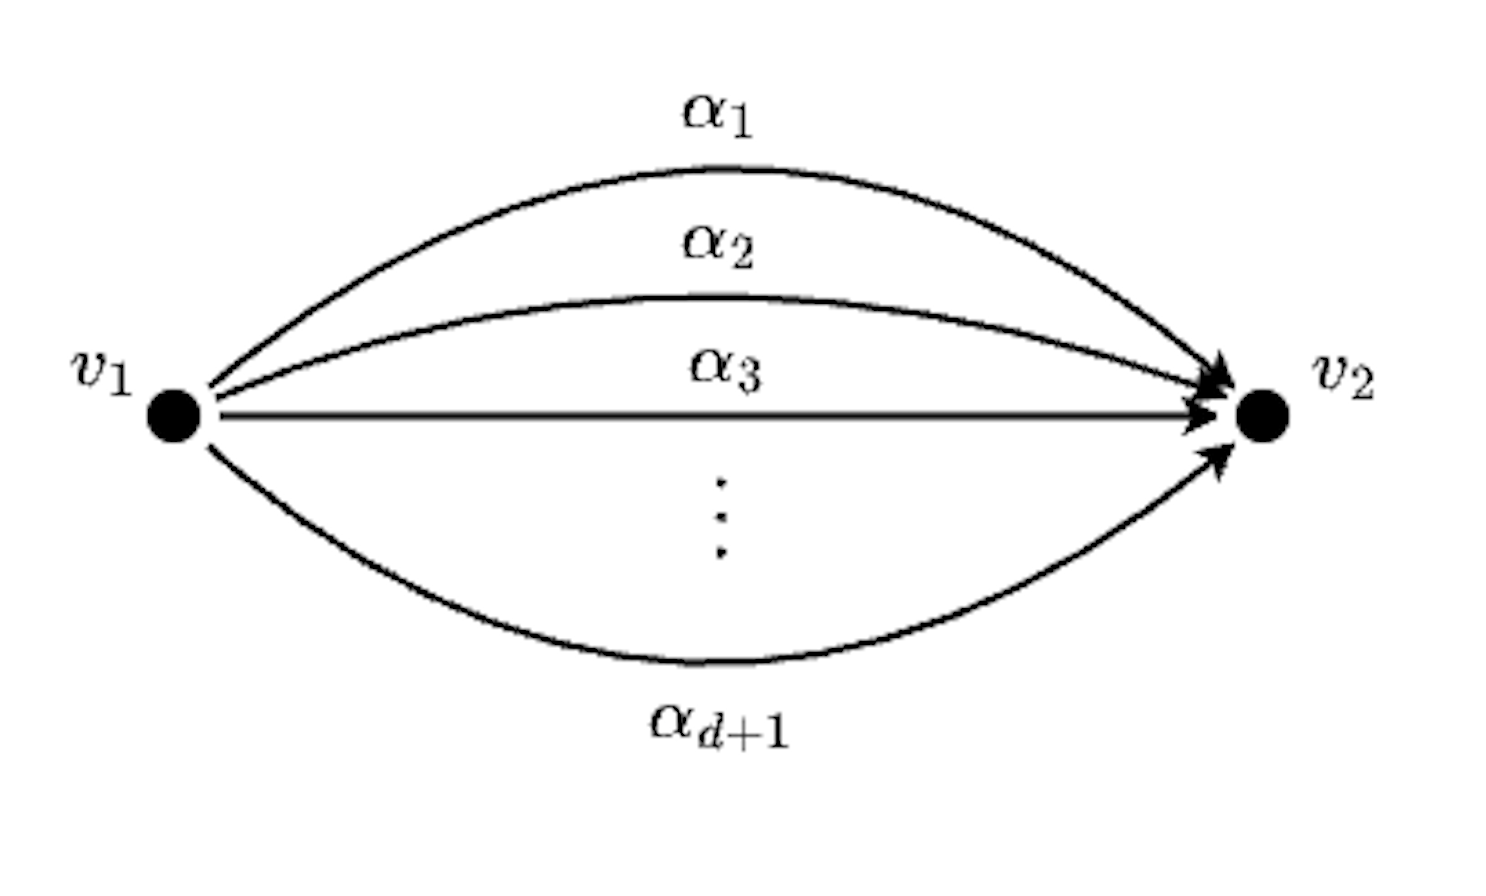
\includegraphics[width=0.4\linewidth]{d+1-quiv.png}
    \caption{}
    \label{d-quiv}
\end{figure}
 
We now wish to inspect the cone of weights equivariant under the action of any subgroup $G \leq \aut(Q)$, which we denote $C_Q^G$, and the relevant walls within this cone. It is not difficult to see our cone $C_Q^G$ is a slice of the cone $C_Q$, that is, 
\begin{align*}
C_Q^G &= C_Q \cap \{\theta \in \hom(Q_0, \Z) \:|\: \theta(v) = \theta(g \cdot v), \;\;g \in G, \;\;v \in Q_0\} \\
&= C_Q \cap \hom(Q_0, \Z)^G.
\end{align*}
The latter set in the intersection is a hyperplane given by the condition that two vertices have the same weight if the vertices lie in the same orbit of $Q_0$ under action by $G$. Since $C_Q^G \subset C_Q$, it is obvious that walls of $C_Q$ that intersect $C_Q^G$ will emerge as walls in $C_Q^G$. 

Ideally, we want to compute $C_Q^G$ without having to compute all of $C_Q$. To do so, we need a few more tools. We define, for an edge $\alpha \in Q_1$, the integral elementary flow map $e_\alpha \in \hom(Q_1, \Z)$ by
\[
e_\alpha(\beta) := \begin{dcases}
    1, &\beta = \alpha \\
    0, &\beta \neq \alpha
\end{dcases}\;.
\]
Let $\{e_\alpha\}_{\alpha \in Q_1}$ be the standard $\Z$-basis vectors of $\hom(Q_1, \Z)$. Then, if $x \in \hom(Q_1, \Z)$, 
    \[
    x = \sum_{\alpha \,\in\, Q_1} a_\alpha e_\alpha
    \]
for some constants $a_\alpha$. It is shown in \cite{hille2003quivers} that the cone $C_Q$ is generated by the rays $I_Q(e_\alpha)$ for all primitive edges $\alpha$. A primitive edge is defined to be an edge $\alpha$ in $Q_1$ for which all directed paths from $\alpha^-$ to $\alpha^+$ contain $\alpha$. We will show a similar result in Proposition \ref{equivariant-cone-generators} for $C_Q^G$ where instead of primitive edges, orbits of $G$ of primitive edges will produce rays that generate the cone. 

\begin{proposition}
    An edge $\alpha$ of $Q$ is primitive if and only if all edges in the orbit $G \cdot \alpha$ are primitive.
\end{proposition}

\begin{proof}
    This is equivalent to saying that automorphisms of $Q$ send primitive arrows to primitive arrows, that is, $\alpha \in Q_1$ is primitive exactly when $g \cdot \alpha$ is primitive. To show this, we suppose the edge $\alpha = \{\alpha^-, \alpha^+\}$ is \textit{not} primitive, meaning there exists a directed path $\alpha^-, v_1, \ldots, v_k, \alpha^+$ such that the sequence $\alpha^-$, $\alpha^+$ does not exist somewhere within the path. If $g$ is an automorphism of $Q$, then $g$ preserving the direction of edges and adjacency relations means that $g \cdot \alpha^-, g \cdot v_0, \ldots, g \cdot v_k, g \cdot \alpha^+$ is a path in $g \cdot Q \cong Q$. This is a path from the vertex $g \cdot \alpha^-$ to the vertex $g \cdot \alpha^+$ that does not contain the sequence $g \cdot \alpha^-$, $g \cdot \alpha^+$. Thus, $g \cdot \alpha$ is not primitive, and $g$ an automorphism (bijective, and thus having inverse) means that primitive arrows must be sent to primitive arrows, too.
\end{proof}

The above proposition means it is sensible to define the following:

\begin{definition}
    If the edges of an orbit $\mathcal{O} \in Q_1 / G$ are primitive then we say the orbit is primitive. If the edges are not primitive, then we say $\mathcal{O}$ is not primitive.
\end{definition}

\begin{proposition} \label{equivariant-cone-generators}
    Let $G \leq \aut(Q)$. The cone of equivariant weights $C_Q^G$ is minimally generated by the rays 
\[
\phi_\mathcal{O} := I_Q\Big(\sum_{\alpha \,\in \,\mathcal{O}}e_\alpha\Big) 
\]
    where $\mathcal{O} \in Q_1 / G$ is a primitive orbit. If $\mathcal{O}$ is not primitive, then the corresponding ray $\phi_\mathcal{O}$ is a linear combination of rays corresponding to primitive orbits.
\end{proposition}

\begin{proof}  
    Let $\theta \in C_Q^G$. Then, there exists an $G$-invariant flow $x$ such that $I_Q(x) = \theta$ and $x(\alpha) \geq 0$ for all $\alpha \in Q_1$. Then, we can express $x = \sum_{\mathcal{O}} a_\mathcal{O} \sum_{\alpha \in \mathcal{O}} e_\alpha$ for some constants $\alpha_\mathcal{O} \geq 0$ where $\mathcal{O} \in Q_1/G$. Using that $I_Q$ is linear,
    \begin{align*}
    \theta &= I_Q\Big(\sum_{\mathcal{O} \,\in\, Q_1/\aut(Q)}a_{\mathcal{O}} \sum_{\alpha \,\in\, \mathcal{O}} e_\alpha \Big) \\ 
    &= \sum_{\mathcal{O} \,\in\, Q_1/\aut(Q)}a_{\mathcal{O}} I_Q\Big(\sum_{\alpha \,\in\, \mathcal{O}} e_\alpha \Big) \\
    &= \sum_{\mathcal{O} \,\in\, Q_1/\aut(Q)} a_\mathcal{O}\phi_\mathcal{O}
    \end{align*}
    Using the same argument as in Hille, we can show the rays $\phi_\mathcal{O}$ where $\mathcal{O}$ is not primitive  are themselves equal to the sum of rays corresponding to primitive orbits. Namely, if $\mathcal{O}'$ is not primitive, then
    \[
    \phi_{\mathcal{O}'} = \sum_{\mathcal{O} }\phi_\mathcal{O}
    \]
    where $\mathcal{O}$ are the orbits that contain the edges in the paths that must exist since the edges in $\mathcal{O}'$ are not primitive. If some of these orbits are not primitive, they can be decomposed further into primitive orbits themselves.
\end{proof}

As mentioned, Hille shows that the possible walls of $C_Q$ correspond exactly to partitions of $Q_0$ into two sets. The natural analogue to our setting would be that the walls of $C_Q^G$ correspond to the partitions of the orbits $Q_0/G$. While the partitions do imply the existence of a possible wall, the converse does not generally hold for $C_Q^G$, as shown in Example \ref{vertex-partition-counterexample}.

\begin{proposition} \label{wall-orbit-partition}
    Every partition of $Q_0 / \aut(Q)$ into two nonempty sets defines a possible wall in $C_Q^{\aut(Q)}$.
\end{proposition}

\begin{proof}
    A partition of $Q_0 / \aut(Q)$ is itself a partition of the vertices, and thus corresponds to a possible wall in $C_Q$.
\end{proof}

\begin{example} \label{vertex-partition-counterexample}
    Consider the quiver $Q$ shown to the left in Figure \ref{quiver-cone-example}. We first compute the unrestricted weight space $C_Q$, which we will see is the three-dimensional cone whose two-dimensional projection is shown on the right in Figure \ref{quiver-cone-example}. By recognizing edges 3, 4, 5, and 6 are primitive edges and determining possible walls via partitions of $Q_0$ into two sets, we arrive with $C_Q$ where $\phi_i$ are the rays corresponding to $I_Q(e_i)$ $(i \in Q_1)$ and the (thin) lines between the rays are the possible walls. Note the bolded line within the cone is not a wall, but rather $C_Q^{\aut(Q)}$, which we will compute now. Via swapping vertex $b$ and $d$ and swapping edges 3 and 4 in $Q$, we can determine that $\aut(Q) \cong S^2 \times S^2$. Under this action, the primitive orbits are the orbit consisting of edges 3 and 4 and the orbit consisting of edges 5 and 6. The corresponding rays are $\phi_3 + \phi_4$ and $\phi_5 + \phi_6$ and are depicted in Figure \ref{quiver-cone-example} as the left-most gray dot and the right-most gray dot, respectively. These two minimally generate $C_Q^{\aut(Q)}$ as per Proposition \ref{equivariant-cone-generators} and so the bolded line is exactly $C_Q^{\aut(Q)}$. To determine the walls, we determine the possible partitions of $Q_0 /\aut(Q) = \{\{a\}, \{b, d\}, \{d\}\}$ into two nonempty sets. These determine 3 walls in $C_Q^{\aut(Q)}$, depicted by the three gray dots in the figure. However, there is a fourth possible wall inside of $C_Q^{\aut(Q)}$ where the two thin lines intersect over the bolded line. Moreover, direct calculation of the polytopes on both sides of the wall verify that the polytopes are indeed different and thus the wall is indeed realized in the cone. It is not determined by a partition of $Q_0 /\aut(Q)$, so the converse of Proposition \ref{wall-orbit-partition} cannot hold.
    

\end{example}

\begin{figure} 
    \centering
    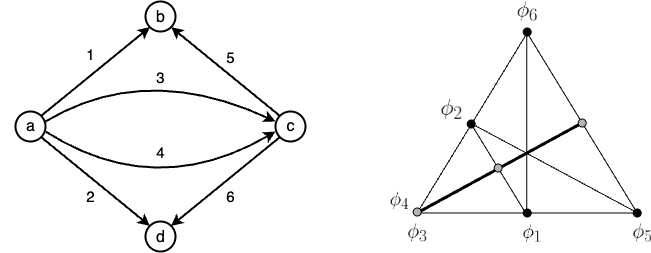
\includegraphics[width=0.7\linewidth]{wall-decomp-example.drawio.png}
    \caption{}
    \label{quiver-cone-example}
\end{figure}

As we will show in Theorem \ref{thm:quotient-graph-correspondence}, the partitions of $Q_0/G$ for any $G \leq \aut(Q)$ correspond bijectively with the possible walls in $C_Q^G$ if we consider only a subset of each polytope, namely the $G$-invariants of $\Delta(Q, \theta)$.

\begin{definition}
    Let $G \leq \aut(Q)$ and $\theta$ be equivariant under $G$. We define $\Delta(Q, \theta)^G$ to be the points of the polytope $\Delta(Q, \theta)$ fixed by all elements of $G$. That is,
    \[
    \Delta(Q, \theta)^G := \{x \in \Delta(Q, \theta) \:|\: (g \cdot x)(\alpha) = x(\alpha) \text{ for all } g \in G\}.
    \]
\end{definition}

Let $I_Q^G$ be the restriction of $I_Q$ to
$\hom(Q_1, \Z)^G$, the set of flows invariant under the action of $G$. It follows that the fibers of each $\theta \in C_Q^G$ under $I_Q^G$ are exactly the sets $\Delta(Q, \theta)^G$. In fact, $\Delta(Q, \theta)^G$ is itself a convex polytope; this follows from the fact that the fixed points of any affine mapping (geometric automorphisms of polytopes are exactly affine mappings) form an affine subset, and the intersection of an affine subset with a polytope is another polytope. We now show this polytope is realized as the polytope for the quotient graph with some weight.

\begin{definition}
    Let $G \leq \aut(Q)$. The quotient quiver $Q/G$ is the quiver realized by taking the quotient of the underlying directed multigraph by $G$. The vertices are orbits of the action of $G$ on $Q_0$ (elements of $Q_0/G$), and a directed edge $(\mathcal{O}_1, \mathcal{O}_2) \in Q_0/\aut(Q) \times Q_0/\aut(Q)$ is an edge in $Q/G$ if there exists some $u \in \mathcal{O}_1$ and $v \in \mathcal{O}_2$ such that $(u, v) \in Q_1$. 
\end{definition}

The obvious canonical projections 
\begin{align*}
    \pi_0 : Q_0 \longrightarrow (Q/G)_0 := Q_0/G \\
    \pi_1 : Q_1 \longrightarrow (Q/G)_1 := Q_1/G
\end{align*}
induce the two maps of weights and flows
\begin{align*}
    \bar \pi_0 &: \hom(Q_0, \Z)^G \longrightarrow \hom((Q/G)_0, \Z), \qquad \bar\pi_0(\theta)(v) = \sum_{w \,\in\, \pi_0^{-1}(v)}\theta(w) \qquad (v \in (Q/G)_0) \\
    \bar\pi_1 &: \hom(Q_1, \Z)^G \longrightarrow \hom((Q/G)_1, \Z), \qquad \bar\pi_1(x)(\alpha) = \sum_{\beta \,\in\, \pi_1^{-1}(\alpha)}x(\beta) \qquad (\alpha \in (Q/G)_1)
\end{align*}
which can both be easily checked to be linear isomorphisms. Moreover, since we require the weight and flows to be $G$-invariant, it follows that $\bar \pi_0(\theta)(v) = |\pi_0^{-1}(v)| \cdot \theta(w)$ for any $w \in \pi_0^{-1}(v)$ and $\bar\pi_1(x)(\alpha) = |\pi_1^{-1}(\alpha)| \cdot x(\beta)$ for any $\beta \in \pi_1^{-1}(\alpha)$. In particular, this means that $\bar\pi_1$ restricts to a mapping on the nonnegative coordinate space $\hom(Q_1, \R_{\geq 0})^G \longrightarrow \hom((Q/G)_1, \R_{\geq 0})$.

\begin{proposition} \label{quotient-acyclic}
    Suppose $G \leq \aut(Q)$. If $Q$ is acyclic, then $Q/G$ is acyclic.
\end{proposition}

\begin{proof}
    Suppose $Q/G$ is cyclic. Thus, there exists a cycle $v_1, v_2, \ldots, v_k =v_1$ in $Q/G$. We now construct a cycle in $Q$. Let $c_1 \in Q_0$ such that $\pi_0(c_1) = v_1$. Since $(v_1, v_2)$ is an edge in $(Q/G)_1$, there must exist at least one edge from a vertex $u_1 \in \pi_0^{-1}(v_1)$ to a vertex $u_2 \in \pi_0^{-1}(v_2)$. Since $u_1$ and $c_1$ lie in the same orbit, we have that $c_1$ is the image of a graph automorphism $g$ sending vertex $u_1$ to $c_1$. Then, there exists an edge starting at $c_1$ and ending at $c_2:= g \cdot u_2$, which is necessarily in $\pi_0^{-1}(u_2)$. Performing this process again at $c_2$ produces an edge from $c_2$ to $c_3$ such that $c_3 \in \pi_0^{-1}(v_3)$. After $k - 1$ iterations, this will produce a path $c_1, c_2, \ldots, c_k$ such that $\pi_0(c_k) = \pi_0(c_1) = v_1$. If $c_1 = c_k$, we are done; this is a cycle in $Q$. If not, repeat the entire process again starting at $c_k$ to construct a path $c_1, \ldots, c_k, c_{k+1}, \ldots, c_{2k}$ such that $\pi_0(c_{2k}) = \pi_0(c_k) = \pi_0(c_1) = v_1$. Since $Q$ is finite by assumption, $\pi_0^{-1}(v_1)$ is finite as well; thus, after some number of iterations of the above process (at maximum $|\pi_0^{-1}(v_1)|$ iterations), we will create a cycle in $Q$. Then, $Q$ must be cyclic.
\end{proof}

The above result means $\Delta(Q/G, \theta)$ is a polytope, nonempty exactly when $\theta \in C_{Q/G}$.

\section{Proof of Theorem \ref{thm:quotient-graph-correspondence}}
\begin{proof}
    Recall $I_Q^G$ was defined above to be $I_Q$ restricted to the space of $G$-invariant flows $\hom(Q_1, \Z)^G$. It is obvious that $I_Q^G$ maps into the space of $G$-invariant weights $\hom(Q_0, \Z)^G$. Let $I_{Q/G} : \hom((Q/G)_1, \Z) \longrightarrow \hom((Q/G)_0, \Z)$ be the incidence map of the quotient quiver $Q/G$. We thus have the following diagram, which we will show commutes.

    % https://q.uiver.app/#q=WzAsNCxbMCwwLCJcXGhvbV9HKFFfMSwgXFxSKSJdLFswLDIsIlxcaG9tKChRL0cpXzEsIFxcUikiXSxbMiwwLCJcXGhvbV9HKFFfMCwgXFxSKSJdLFsyLDIsIlxcaG9tKChRL0cpXzAsIFxcUikiXSxbMCwxLCJcXGJhclxccGlfMSIsMl0sWzAsMiwiSV9RXkciXSxbMSwzLCJJX3tRL0d9Il0sWzIsMywiXFxiYXJcXHBpXzAiLDJdXQ==t
\[\begin{tikzcd}
	{\hom(Q_1, \Z)^G} && {\hom(Q_0, \Z)^G} \\
	\\
	{\hom((Q/G)_1, \Z)} && {\hom((Q/G)_0, \Z)}
	\arrow["{I_Q^G}", from=1-1, to=1-3]
	\arrow["{\bar\pi_1}"', from=1-1, to=3-1]
	\arrow["{\bar\pi_0}"', from=1-3, to=3-3]
	\arrow["{I_{Q/G}}", from=3-1, to=3-3]
\end{tikzcd}\]
Take $x \in \hom(Q_1, \Z)^G$, and for any vertex $v \in (Q/G)_0$,
\begin{align*}
    I_{Q/G}(\bar\pi_1(x))(v) &= \sum_{\alpha \,\in\, (Q/G)_1\:|\: \alpha^+ \,=\,v} \bar\pi_1(x)(\alpha) - \sum_{\alpha \,\in\, (Q/G)_1\:|\: \alpha^-\,=\,v} \bar\pi_1(x)(\alpha) \\
    &= \sum_{\alpha \, \in\, (Q/G)_1\:|\: \alpha^+ \,=\,v} |\pi_1^{-1}(\alpha)|\cdot x(\beta_\alpha) - \sum_{\alpha \,\in\, (Q/G)_1\:|\: \alpha^-\,=\,v}  |\pi_1^{-1}(\alpha)|\cdot x(\beta_\alpha)
\end{align*}
where $\beta_\alpha \in \pi_1^{-1}(\alpha)$. Then, for any $\alpha \in (Q/G)_1$, note that $|\pi_1^{-1}(\alpha)|$ is a multiple of $|\pi_0^{-1}(v)|$ because each vertex $w \in \pi_0^{-1}(v)$ must have the same number of ingoing (or outgoing) edges in $\pi_1^{-1}(\alpha)$ as $v$ does due to automorphisms preserving edge count and orientation. Thus, supposing $|\pi_1^{-1}(\alpha)| = k_\alpha|\pi_0^{-1}(v)|$ for all $\alpha$, the integer $k_\alpha$ counts the number of edges entering (or exiting) $w$ that are in the orbit that maps to $\alpha$ by $\pi_1$. We can then write
\[
= \sum_{\alpha \, \in\, (Q/G)_1\:|\: \alpha^+ \,=\,v} k_\alpha|\pi_0^{-1}(v)|\cdot x(\beta_\alpha) - \sum_{\alpha \,\in\, (Q/G)_1\:|\: \alpha^-\,=\,v}  k_\alpha|\pi_0^{-1}(v)|\cdot x(\beta_\alpha).
\]
On the other hand, we have for any vertex $v \in (Q/G)_0$,
\begin{align*}
    \bar\pi_0(I_Q^G(x))(v) &= |\pi_0^{-1}(v)|\cdot I_Q^G(x)(w_v) \\
    &= \sum_{\beta \, \in\, Q_1\:|\: \beta^+ \,=\,w_v} |\pi_0^{-1}(v)|\cdot x(\beta) - \sum_{\beta \,\in\, Q_1\:|\: \beta^-\,=\,w_v} |\pi_0^{-1}(v)|\cdot x(\beta)
\end{align*}
where $w_v \in \pi_0^{-1}(v)$. We can change our sum to sum over all edges $\alpha \in (Q/G)_1$ that are entering $v$ if we simultaneously sum over each edge in the orbit $\pi_1^{-1}(\alpha)$ that are incident to $w_v$.  However, since each edge in the orbit has constant flow, we can replace the second sum with $k_\alpha\cdot x(\beta_\alpha)$ for some element $\beta_\alpha \in \pi_1^{-1}(\alpha)$ where $k_\alpha$ can be seen to be the same constant as used previously. Thus, we have
\begin{align*}
\sum_{\beta \, \in\, Q_1\:|\: \beta^+ \,=\,w_v} |\pi_0^{-1}(v)|\cdot x(\beta) &= \sum_{\alpha \, \in\, (Q/G)_1\:|\: \alpha^+ \,=\,v} \left(\sum_{\beta \, \in\, \pi_1^{-1}(\alpha) \:|\: \beta^+ \,=\,w_v} |\pi_0^{-1}(v)|\cdot x(\beta) \right)\\
&= \sum_{\alpha \, \in\, (Q/G)_1\:|\: \alpha^+ \,=\,v} k_\alpha|\pi_0^{-1}(v)|\cdot x(\beta_\alpha)
\end{align*}
and the same holds for edges exiting $v$. Hence, 
\[
    I_{Q/G}(\bar\pi_1(x))(v) = \sum_{\alpha \, \in\, (Q/G)_1\:|\: \alpha^+ \,=\,v} k_\alpha|\pi_0^{-1}(v)|\cdot x(\beta_\alpha) - \sum_{\alpha \,\in\, (Q/G)_1\:|\: \alpha^-\,=\,v}  k_\alpha|\pi_0^{-1}(v)|\cdot x(\beta_\alpha) = \bar\pi_0(I_Q^G(x))(v)
\]
and so the diagram commutes.

Since $Q/G$ is acyclic via Proposition \ref{quotient-acyclic}, $\Delta(Q/G, \bar\pi_0(\theta))$ defined by the intersection $ I_{Q/G}^{-1}(\bar\pi_0(\theta))\cap \hom((Q/G)_1, \Z_{\geq0})$ is indeed a polytope. We now show $\bar\pi_1(\Delta(Q, \theta)^G) = \Delta(Q/G, \bar\pi_0(\theta))$ via two-way inclusion. Using the diagram above, 
\begin{align*}
    (I_{Q/G} \circ \bar\pi_1)(\Delta(Q, \theta)^G) = (\bar\pi_0\circ I_Q^G)(\Delta(Q, \theta)^G)
\end{align*}
yielding $\bar\pi_1(\Delta(Q, \theta)^G)\subseteq I_{Q/G}^{-1}(\bar\pi_0(\theta))$. Since $\bar\pi_1$ restricts to an isomorphism on $\hom(Q_1, \Z_{\geq0})^G$ to $\hom((Q/G)_1, \Z_{\geq 0})$ and $\Delta(Q, \theta)^G \subset \hom(Q_1, \Z_{\geq0})^G$, we get the one-way inclusion
\[
\bar\pi_1(\Delta(Q, \theta)^G) \subseteq I_{Q/G}^{-1}(\bar\pi_0(\theta)) \cap \hom((Q/G)_1, \Z_{\geq 0}) = \Delta(Q/G, \bar\pi_0(\theta)).
\]
To show the reverse inclusion, use the diagram to write
\[
(I_Q^G \circ \bar\pi^{-1}_1)(\Delta(Q/G, \bar\pi_0(\theta)) = (\bar\pi_0^{-1} \circ I_{Q/G})(\Delta(Q/G, \bar\pi_0(\theta))
\]
yielding $\bar\pi^{-1}_1(\Delta(Q/G, \bar\pi_0(\theta)) \subseteq (I_Q^G)^{-1}(\theta)$. Similarly, $\bar\pi_1^{-1}$ restricts to an isomorphism on $\hom((Q/G)_1, \Z_{\geq 0})$ to $\hom(Q_1, \Z_{\geq0})^G$ giving
\[
\bar\pi^{-1}_1(\Delta(Q/G, \bar\pi_0(\theta)) \subseteq (I_Q^G)^{-1}(\theta)\cap \hom(Q_1, \Z_{\geq0})^G = \Delta(Q, \theta)^G,
\]
or $\Delta(Q/G, \bar\pi_0(\theta) \subseteq \bar\pi_1(\Delta(Q, \theta)^G)$. Thus, $\bar\pi_1(\Delta(Q, \theta)^G) = \Delta(Q/G, \bar\pi_0(\theta))$. Since $\bar\pi_1$ is a linear isomorphism, we have that the image of an affine subspace is the affine span of the image. Hence, $\bar\pi_1(\aff(\Delta(Q, \theta)^G)) = \aff(\bar\pi_1(\Delta(Q, \theta)^G)) = \aff(\Delta(Q/G, \bar\pi_0(\theta)))$ and so $\bar\pi_1$ clearly restricts to an isomorphism between the affine spaces, the polytopes, and the lattice points of the polytope (since $\bar\pi_1$ is an integral map). Thus, $\Delta(Q, \theta)^G \cong \Delta(Q/G, \bar\pi_0(\theta)).$

Finally, for the weight cones, we have
\begin{align*}
    \bar\pi_0(C_Q^G) &= \bar\pi_0(I_Q^G(\hom(Q_1, \Z_{\geq 0})^G)) \\ 
    &= I_{Q/G}(\bar\pi_1(\hom(Q_1, \Z_{\geq 0})^G)) \\ 
    &= I_{Q/G}(\hom((Q/G)_1, \Z_{\geq 0})) \\
    &= C_{Q/G}.
\end{align*}
completing the proof.
\end{proof}

\section{Tightening Quivers with Canonical Weight}

The canonical weight $\delta_Q$ of a quiver $Q$ is the image under $I_Q$ of the flow of all 1's. Much study has gone into the polytopes associated with quivers along with their canonical weight, especially since the polytope of the canonical weight is known to be reflexive. For example, \cite{domokos2016equations} and others demonstrate that there are only five polytopes that arise from quivers with first Betti number 2 up to integral-affine isomorphism. In this section, we present four different graph operations that can be used to completely tighten an arbitrary quiver with respect to its canonical weight.

\begin{definition}
    A tightening operation is a graph operation performed on $Q$ that takes the quiver $Q$ to another quiver $\hat Q$ such that $|\hat Q_1| < |Q_1|$ and $\Delta(Q, \delta_Q) \cong \Delta(\hat Q, \delta_{\hat Q})$. A quiver $Q$ is called tight if no tightening operations can be performed on $Q$.
\end{definition}

It is important to note that in this section, we are solely tightening with respect to the canonical weight. Also, it is immediate by definition that every quiver can be ``tightened'' via repeated tightening operations to a tight form. The only tightening operations we will need are the two well-known operations presented below.

\begin{definition} We define two simple graph operations below. Recall that the contraction of an edge $\alpha = (\alpha^- , \alpha^+)$ in $Q$ is the gluing of the vertices $\alpha^-$ and $\alpha^+$ followed by the removal of $\alpha$.
\begin{itemize}
    \item[(i)](Pruning)
    Given a quiver $Q$, define $\hat Q$ as the quiver gained by contracting an edge of $Q$ that is not contained in any underlying undirected cycle of $Q$.
    \item[(ii)](Path Contraction)
    Suppose $v$ is a vertex in $Q$ of in-degree 1 and out-degree 1. Define $\hat Q$ as the quiver gained by contracting either one of the edges incident to $v$.
\end{itemize}
\end{definition}

\begin{figure}[h!bt]
        \centering
        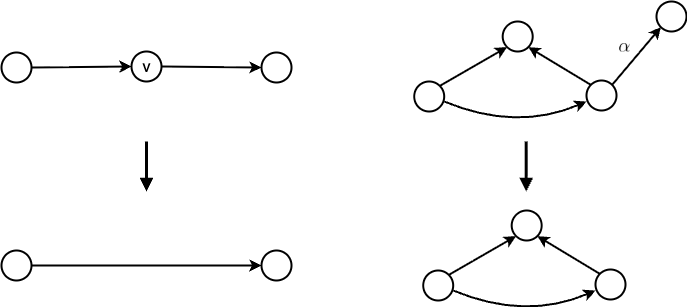
\includegraphics[width=0.5\linewidth]{graph_operations.png}
        \caption{The graph operations path contraction (left) and pruning (right).}
        \label{fig:placeholder}
\end{figure}

\begin{proposition}
    Pruning and path contraction are tightening operations.
\end{proposition}

\begin{proof}
    Can be trivially devised from Proposition 3.7 and Corollary 3.8, respectively, in \cite{domokos2016equations}.
\end{proof}

The next operation we present allows us to understand the polytope of a quiver through the product of the polytopes of two subquivers that meet at just one vertex. Recall that the wedge sum of two quivers $Q$ and $P$, denoted $Q \vee P$, is the quiver arising from taking the disjoint union of $Q$ and $P$ and gluing them together at exactly one vertex.
The below result was known in \cite{domokos2016equations}.

\begin{proposition} (Cut-Vertex Decomposition)
    If $Q$ and $Q'$ are two quivers, then $\Delta(Q \vee Q', \delta_{Q \vee Q'}) \cong \Delta(Q, \delta_Q) \times \Delta(Q', \delta_{Q'})$.
\end{proposition}

\begin{proof}
    Any flow $x \in \Delta(Q \vee Q', \delta_{Q \vee Q'})$ uniquely decomposes as $x = y + y'$ for some flows $y \in \Delta(Q, \delta_Q)$ and $y' \in \Delta(Q', \delta_{Q'})$. Thus, the map $\Delta(Q \vee Q', \delta_{Q \vee Q'}) \longrightarrow \Delta(Q, \delta_Q) \times \Delta(Q', \delta_{Q'})$, $x \mapsto (y, y')$ is clearly a restriction of an (integral) linear isomorphism of the affine spaces in which they lie. Hence, it is an integral-affine isomorphism.
\end{proof}

The above result means it is enough to consider quivers without any cut vertices, that is, vertices whose deletion would disconnect the graph. In light of this, we now define our final graph operation but only for quivers without cut vertices.

\begin{definition}
Suppose $Q$ has no cut vertices. Let $C$ be an undirected cycle of $Q$. Fix an undirected path decomposition of $C$ into paths $p_1, \ldots, p_k$, and suppose that each path $p_i$ has terminal vertices $p_i'$ and $p_i''$ for $1 \leq i \leq k$. We define the permutable subquiver of $p_i$, denoted $R_{p_i}$, to be the subquiver of $Q$ realized by the union of all undirected paths connecting $p_i'$ and $p_i''$ that are contained in $Q - (C - p_i)$, the subgraph of $Q$ with all vertices and edges of $C$ outside of $p_i$ removed. That is, if $Q^c_{p_i} := Q - (C - p_i)$ and $\gamma$ is an undirected path between $p_i'$ and $p_i''$,
\[
R_{p_i} := \bigcup_{\gamma \,\subset\, Q^c_{p_i}}\gamma
\]
with orientations on $R_{p_i}$ inherited from $Q$.
This produces a collection of generally nondisjoint subquivers $\mathcal{R}_C := \{R_{p_i}\}^k_{i=1}$ of $Q$.
We say $\mathcal{R}_C$ is permutation-ready if
\begin{itemize}
    \item[(i)] $R_{p_i} \cap R_{p_j} = p_i \cap p_j$ for all distinct pairs $R_{p_i}, R_{p_j} \in \mathcal{R}_C$
    \item[(ii)]$\bigcup_{R_{p_i} \,\in\,\mathcal{R}_C }R_{p_i} = Q$
\end{itemize}
\end{definition}

\begin{definition} \label{subquiver_permutation}
    (Subquiver Permutation) Suppose $Q$ is a quiver, $C \subset Q$ an undirected cycle, and $\mathcal{R}_C$ permutation-ready. Let $R_{p_i}, R_{p_j} \in \mathcal{R}_C$. Further, define an orientation on the cycle $C$ and in an order matching this orientation, denote the terminal vertices of $p_i$ as $v'$ and $v''$ and the terminal vertices of $p_j$ as $u'$ and $u''$. Define $\hat Q$ to be the quiver formed by first taking the disjoint union of $R_{p_i}$, $R_{p_j}$, and $Q' := Q - ((R_{p_i} - \{v', v''\}) \cup (R_{p_j} - \{u', u''\}))$ and then making the following vertex identifications:
    \begin{itemize}
        \item[(i)] $v' \in R_{p_i}$ with $u' \in Q'$
        \item[(ii)] $v'' \in R_{p_i}$ with $u'' \in Q'$
        \item[(iii)] $u' \in R_{p_j}$ with $v' \in Q'$
        \item[(iv)] $u'' \in R_{p_j}$ with $v'' \in Q'$.
    \end{itemize}
    We say $\hat Q$ is the quiver resulting from permuting subquivers $R_{p_i}$ with $R_{p_j}$.
\end{definition}

\begin{conjecture}
    Suppose $Q$ is a quiver, $C \subset Q$ an undirected cycle or path, and $\mathcal{R}_C$ permutation-ready. For any $R_{p_i},\,R_{p_j} \in \mathcal{R}_C$, let $\hat Q$ be the quiver formed by permuting subquivers $R_{p_i}$ and $R_{p_j}$. Then, $\hat Q$ is an acyclic quiver, and $\Delta(Q, \delta_Q) \cong \Delta(\hat Q, \delta_{\hat Q})$.
\end{conjecture}

\begin{proof}
    
\end{proof}

The following necessary and sufficient condition for the tightness of a quiver with canonical weight is given in \cite{domokos2016equations}. We use it to show our three operations are enough to reduce any quiver with canonical weight to a tight form.

\begin{proposition}\label{canonical-contraction-condition}
    (Joó-Domokos) Given a connected quiver $Q$ the pair $(Q, \delta_Q)$ is tight if and only if there is no partition $Q_0 = S \sqcup S'$ such that there is at most one arrow from $S$ to $S'$ and there is at most one arrow from $S'$ to $S$.
\end{proposition}

\begin{proposition}
    Every quiver $Q$ can be tightened via a finite number of prunes, path contractions, and subquiver permutations.
\end{proposition}

\begin{proof}
    We show that Proposition \ref{canonical-contraction-condition} holds exactly when we can find two permutable subquivers such that their permutation results in a quiver with an arrow contractable via either pruning or chain contraction. For the forward direction, suppose such a decomposition exists. We prove this in two cases. First, let $Q_0 = S \sqcup S'$, $\alpha$ be an arrow from $S'$ to $S$, and no other arrow between the two sets. Take $C$ to be an undirected path containing $\alpha$, say $c_1, \ldots, c_n$ starting in $S'$ and ending in $S$. Decompose it into three paths $p_1 = (c_1, c_2,  \ldots, c_k = \alpha^-)$, $p_2 = (\alpha^-, \alpha^+)$, and $p_3 = (\alpha^+ = c_k, c_{k+1}, \ldots, c_n)$. Produce from this undirected path decomposition of $C$ the subquiver collection $\mathcal{R}_C$ and see that it is permutation-ready, owing to $\alpha$ being a bridge between $S'$ and $S$. Then, let $\hat{Q}$ be the quiver produced by subquiver-permuting $R_{p_2}$ and $R_{p_3}$. By construction, $R_{p_2}$ is either an edge leading to a leaf vertex or an edge leading to a tree structure, that is, there are no undirected loops past this bridge. In either case, $\hat Q$ can be pruned to remove $\alpha$.
    
    % such a decomposition exists; that is, suppose $Q_0 = S \sqcup S'$ with $\alpha$ an arrow from $S$ to $S'$ and another arrow $\beta$ from $S'$ to $S$, as in Figure \ref{tightenquiv-case-1}. Let $P \subset Q$ be the permutable subquiver induced by vertices $\alpha^-$ and $\beta^+$ without $\alpha^+$ if $\beta$ exists or by $\alpha^-$ and some $v \in S \setminus \{\alpha^-\}$ without $\alpha^+$ otherwise. Similarly, let $R \subset Q$ be the permutable subquiver induced by vertices induced by $\alpha^-$ and $\alpha^+$ without $\beta^+$ if $\beta$ exists or by $\alpha^-$ and $\alpha^+$ without $v$, otherwise. 
    
    In a similar way, $P$ is exactly the induced subgraph of the set of vertices in a tree incident to $\alpha^-$ or $\beta^+$ (or $v$ if $\beta$ does not exist). This follows from every edge in $Q[\hat{S}]$ being part of a path from $\alpha^-$ to $\beta^+$ or part of a tree incident to a non-terminal vertex in such a path. In the same way, any vertex in $S'$ cannot be part of a path from $\alpha^-$ to $\beta^+$ (or $v$ if $\beta$ does not exist) since any undirected path containing any vertex in $S'$ must necessarily contain $\alpha^+$.

    Notably, $P \cap R = \{\alpha^-\}$ and so $P$ and $R$ permute. Then, we can define $\widetilde{Q}$ as the resulting quiver after permuting $P$ and $R$ and apply Proposition \ref{subquiver_permutation} to see $\Delta(Q, \delta_Q)$ is integral-affinely isomorphic to $\Delta(\widetilde{Q}, \delta_{\widetilde{Q}})$. At this point, $\widetilde{Q}$ resembles one of the two cases below on the right. If $\beta$ exists, $\alpha$ can be contracted via chain contraction. Otherwise, pruning contracts $\alpha$. In either case, we result with a quiver that with the canonical weight produces a polytope integral-affinely isomorphic to $\Delta(Q, \delta_Q)$.
    \begin{figure}[h!]
    \label{tightenquiv-case-1}
        \centering
        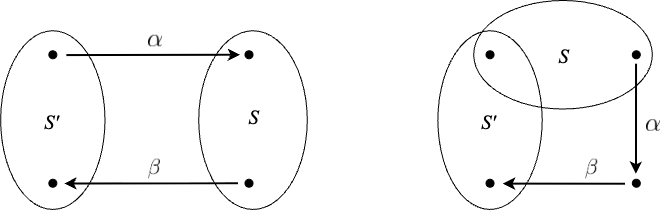
\includegraphics[width=0.75\linewidth]{subquiv_permutation.drawio.png}
    \end{figure}
    If there are more contractible arrows, then Proposition \ref{canonical-contraction-condition} holds and so we can perform subquiver permutation followed by pruning or chain contraction to contract the arrow as explained above. If no more contractible arrows exist, the quiver is tight.
\end{proof}
    
\newpage
\bibliographystyle{alpha}
\bibliography{references} 

\end{document}
